\documentclass[12pt]{article}
\usepackage{graphicx,tikz,tikz-network,tkz-euclide}
\usepackage{amsfonts,amsmath,amssymb}
\title{Math Club Fifth Week Solutions}
\usetikzlibrary {positioning}

\parindent 0pt
\date{October 2024}

\newcounter{problem}
\setcounter{problem}{0}
\newcounter{problemB}
\setcounter{problemB}{0}

\newenvironment{problem}[1]{%
    \stepcounter{problem}
    \noindent\textbf{Problem A\theproblem:} #1
    \\[1em]
}{}

\newenvironment{problemB}[1]{%
    \stepcounter{problemB}
    \noindent\textbf{Problem B\theproblemB:} #1
    \\[1em]
}{}

\newcommand{\multChoice}[5]{%
    \begin{tabular}{l @{\hskip 1.5cm} l @{\hskip 1.5cm} l @{\hskip 1.5cm} l @{\hskip 1.5cm} l}
    A. #1 & B. #2 & C. #3 & D. #4 & E. #5
    \end{tabular}
}

\newenvironment{solution}{%
    \vspace{1em}
    \noindent\textbf{Solution:} 
}{}

\setlength{\baselineskip}{5\baselineskip}
\usetikzlibrary {positioning}
\newcommand{\myVertex}[3]{%
    \Vertex[x=#1,y=#2,size=0.5,label=$#3$,position=90,fontscale=2,style={color=blue}]{#3}
}
\newcommand{\simpleVertex}[3]{%
    \Vertex[x=#1,y=#2,size=0.5,position=180,fontscale=2,style={color=red}]{#3}
}
\newcommand{\invisibleVertex}[3]{%
    \Vertex[x=#1,y=#2,size=0.5,opacity =0,position=180,fontscale=2,style={color=white}]{#3}
}

\begin{document}
\sloppy
\maketitle

\section*{AMATYC problems}

\begin{problem}[A][1][AMATYC Fall 2001/1]
    % Algebra ^ System of Equations ^ Student Math League
    Add \textit{this} to \textit{that}, divide by three; the square of \textit{this} of course you'll see. \\
    But \textit{that} to \textit{this} is eight to one; so find what \textit{this} is, and you're done.
\end{problem}
\multChoice{3}{9}{1/3}{0}{Two of the preceding}

\begin{solution}[A]
    Let \textit{this} $=a$ and \textit{that} $=b$, then $(b:a)=(8:1)$ and
    \begin{align*}
        a^2=\frac{a+b}{3}=\frac{(8a)+a}{3} \\
        \iff a^2 = 3a \iff a=3
    \end{align*}
    Note that $(b:a)=(8:1) \Rightarrow a \neq 0$
\end{solution}

\begin{problem}[A][2][AMATYC Fall 2015/5]
    % System of Equations ^ Student Math League
    Let $p,q$ be two constants for which the equation $2x + p = q$ has the solution $x = 12$. Find the solution to the equation $3x + q = p$.
\end{problem}
 \multChoice{-18}{-8}{-4}{8}{18}

\begin{solution}[B]
    Since $2x+p=q \Rightarrow x=12$ then
    $$q-p = 2 \times 12 = 24$$
    The equation $3x+q=p$ has solution
    $$x = \frac{p-q}{3} = \frac{-24}{3}=-8$$
\end{solution}

\begin{problem}[N][4][AMATYC Fall 2015/4]
    % Divisibility ^ MOD ^ Student Math League
    The students in Ms. Nguyen's 8th grade math class can be seated in rows of 4 or 5, each time with exactly the same number of seats in each row, but when seated in rows of 6, one row has exactly 2 fewer students than all the other rows. If 4 new students join the class, in how many equal rows could her students now be seated? (Assume the class is less than 100 students)
\end{problem}
\multChoice{7}{8}{9}{10}{11}

\begin{solution}[E]
    Let $N$ be the number of students in the class. The smallest number divisible by both 4 and 5 is 20, and we know $N<100$, so $N \in \{20, 40 , 60 , 80\}$. We also know that $N+2$ is divisible by 6, so there must exist some $k \in \mathbb{Z}^+$ such that
    \begin{align*}
        N &= 6k-2\\
        &=6(k-1)+4
    \end{align*}
    Checking the possible cases for $N$, only $40 \equiv 4 \pmod6$. This means that after 4 students join, there are 44 students in the class. Out of the given solutions, only \fbox{11} divides 44 evenly.
\end{solution}

\vskip 1cm

\begin{problem}[N][3][AMATYC Fall 2015/6]
    % Divisibility ^ MOD ^ Inequalities ^ Student Math League
    My piggy bank has 42 coins worth exactly \$1.00. If it has at least one quarter, dime, nickel, and penny, find the total number of dimes and nickels.
   \end{problem}
\multChoice{3}{4}{5}{6}{7}

\begin{solution}[D]
   Let $q,d,n,p \in \mathbb{Z}_{\geq 1}$ be the amount of quarters, dimes, nickels and pennies, respectively. Then
\begin{align}
    q+d+n+p=42 \\
    25q+10d+5n+p=100
\end{align}
Note that (2) means $100>25q \iff 4>q$, thus $q \in \{1,2,3\}$ \\
If $3 \geq q \geq 2$ then 
\begin{align*}
    (1) &\Rightarrow d+n+p \geq 42-3 = 39\\ %\tag{1} \label{eq:1} \\
        &\Rightarrow -d-n-p \leq -39 \\
    (2) &\Rightarrow 10d+5n+p \leq 100 - 25 \times 2 = 50 \
\end{align*}
Adding the inequalities we see that $9d+4n \leq 11$ but since we must have at least one coin of each type we also have $9d+4n \geq 13$ which is a contradiction, meaning $q=1$
\begin{align*}
    (1) &\Rightarrow d+n+p = 41 \\  %\tag{1} \label{eq:1} \\
    (2) &\Rightarrow 10d+5n+p= 75 \\
        &\Rightarrow 9d+4n=34
\end{align*}
We can make the same we did with $q$, in this case $34>9d$ which tell us that $d \in \{1,2,3\}$ \\
But $d \equiv 9d+4n = 34 \equiv 2 \hspace{3pt} (\hspace{-7pt} \mod 4)$ and the only number with this property in $\{1,2,3\}$ is clearly $d=2$, which implies $n=4$, so our answer is 2+4=\boxed{6}

\end{solution}

\vskip 1cm

\begin{problem}[C][4][AMATYC Spring 2010/6]
    % Floor Function ^ Counting ^ Student Math League
    Let $\lfloor x \rfloor$ represent the greatest integer $\leq x$, find 
    $$\lfloor \log_5 1 \rfloor + \lfloor \log_5 2 \rfloor + \ldots + \lfloor \log_5 2010 \rfloor$$
\end{problem}

\begin{solution}[7,264]
    We count how many numbers fall within powers of 5:
    \begin{align*}
        (5-1)(0)+(25-5)(1)+(125-25)(2)+(625-125)(3)+(2011-625)(4)
    \end{align*}
    Summing, we get \fbox{7,264}.
\end{solution}

\vskip 1cm

\begin{problem}[C][5][AMATYC Fall 2014/11]
    % Brute Force ^ Student Math League
    The sequence \(\{a_n\}\) satisfies \(a_n = a_{n-1} + a_{n-3}\) for all \(n \geq 4\). If \(a_1 = 3\) and \(a_6 = 30\), find \(a_8\).
   \end{problem}
\multChoice{63}{66}{69}{72}{75}

\begin{solution}[A]
   First note that
   \begin{align} \setcounter{equation}{0}
       a_8 &= a_7 + a_5\\
       a_6 &= a_5 + a_3
   \end{align}
   You might want to make a similar equation to (2) for $a_1$, but notice that since the given equation only holds for $n \geq 4$. The next best thing is creating some other equation with $a_1$ in it.
   \begin{align}
       a_4=a_3+a_1
   \end{align}
   We want everything in terms of $a_1$ and $a_6$ since we know them. We substitute $a_7=a_6+a_4$ into (1) because it includes $a_6$. We can't do the same with $a_5=a_4+a_2$, unfortunately, because we have no way of knowing what $a_2$ is.
   \begin{align}
       a_8 &= (a_6 + a_4) + a_5
   \end{align}
   So we need $a_4 + a_5$ which you can get by combining (2) and (3).
   \begin{align*}
       a_5 &= a_6 - a_3\\
       +(a_4 &= a_3 + a_1)\\
       a_4 + a_5 &= a_6 + a_1\\
   \end{align*}
   Therefore,
   \begin{align*}
       a_8 &= a_6 + a_4 + a_5\\
       &= 2a_6 + a_1\\
       &=2(30)+3\\
       &=\boxed{63}\\
   \end{align*}
\end{solution}

\begin{problem}[A][4][AMATYC April 1997/6]
   % Algebra ^ Student Math League
   If the solution set for $f(x) < 3$ is $[0,\infty)$, and the solution set for $f(x) > -2$ is $(-\infty, 5)$, then the solution set for $[f(x)]^2 \geq f(x) + 6$ is
\end{problem}

\multChoice{$(-\infty,\infty)$}{$[0,5]$}{$(-\infty,0]$}{$[5,\infty)$ \\}
{$(-\infty,0) \cup [5,\infty)$}

\begin{solution}
   First note that
\begin{align*} \setcounter{equation}{0}
    f^2(x) &\geq f(x)+6\\
    f^2(x)-f(x)-6 &\geq 0 \\
    (f(x)+2)(f(x)-3) &\geq 0
   \end{align*}
   So we want $f(x) \leq -2$ or $f(x) \geq 3$, then we can use the complement of the solutions for $f(x) > -2$ and $f(x)<3$ , since we know them
   \begin{align*}
      f(x) &\leq -2 \Rightarrow x \in \mathbb{R} - (-\infty,5) \equiv [5,\infty) \\
      f(x) &\geq 3 \Rightarrow x \in \mathbb{R} - [0,\infty] \equiv (-\infty,0)
   \end{align*}
   Then $x \in (-\infty,0) \cup [5,\infty)$  $\Box$
\end{solution}

\begin{problem}[C][2][AMATYC Spring 2016/6]
   % Discrete ^ Knights and Knaves ^ Student Math League
   Each member of a group of 5 people is either a knight, who always tells the truth, or a knave, who always lies. Each member of the group looks at everyone else in the group, and then one member says, “I see at least one person who sees only knaves.” What is the least possible number of knights in the group?  
\end{problem}
\multChoice{0}{1}{2}{3}{4}

\begin{solution}[C]
   First we will show that we can't have less than 2 knights, and that having 2 knights is possible, then it would imply that 2 is the least possible amount of knights.\\
   Assume there is at most one knight, fix a person and call it Finn, that can be either a knave or a knight, and that is a knave if and only if there are no knights. Then any knave that is looking at Finn is looking at someone that sees only knaves, since knaves always lies this is not possible \\
   Say that we have two knights, namely Finn and Jake, then both are telling the truth when they say that they see at least one person who sees only knaves, also all the knaves are effectively lying since all the persons they see are seeing at least one knight.\\
   Therefore we can conclude that 2 knights is minimum


\begin{center}
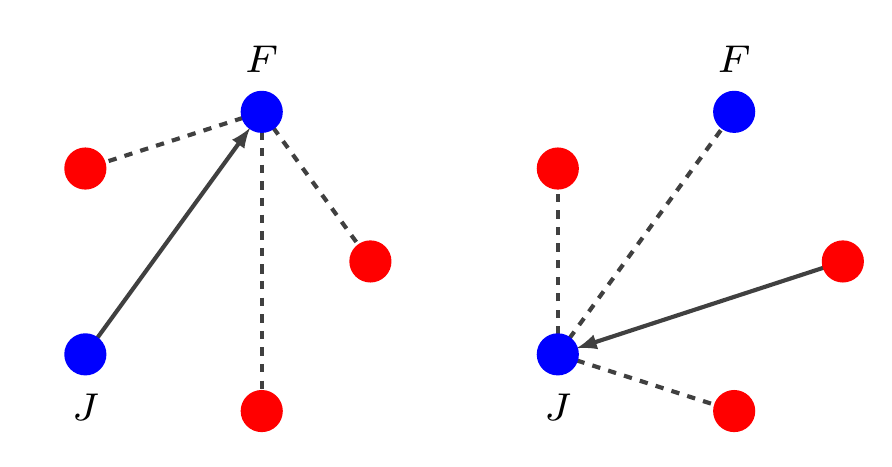
\begin{tikzpicture}
    %v1
    \Vertex[x=-1.62,y=-1.18,size=0.5,label=$J$,position=270,fontscale=2,style={color=blue}]{J}
    \myVertex{0.62}{1.9}{F}
    \simpleVertex{-1.62}{1.18}{L}
    \simpleVertex{2}{0}{L'}
    \simpleVertex{0.62}{-1.9}{L''}
    %v2
    \Vertex[x=4.38,y=-1.18,size=0.5,label=$J$,position=270,fontscale=2,style={color=blue}]{J'}
    \Vertex[x=6.62,y=1.9,size=0.5,label=$F$,position=90,fontscale=2,style={color=blue}]{F'}
    \simpleVertex{4.38}{1.18}{R}
    \simpleVertex{8}{0}{R'}
    \simpleVertex{6.62}{-1.9}{R''}
    %E1
    \Edge[Direct](J)(F)
    \Edge[style={dashed}](F)(L)
    \Edge[style={dashed}](F)(L')
    \Edge[style={dashed}](F)(L'')
    %E2
    \Edge[Direct](R')(J')
    \Edge[style={dashed}](J')(F')
    \Edge[style={dashed}](J')(R)
    \Edge[style={dashed}](J')(R'')   
\end{tikzpicture} 
\end{center}
\end{solution}
\vskip 1cm 

\begin{problem}[N][6][AMATYC Spring 2015/17]
   % MinMax ^ MOD ^ Chinese Remainder Theorem ^ Student Math League
   The sum of the first $n$ positive integers equals the sum of the 5 consecutive
    positive integers starting at $a$ and the sum of the 8 consecutive positive
    integers starting at $b$. Find $a-b$ for the least such $a$ and $b$.
\end{problem}
\multChoice{16}{21}{24}{60}{63}
\begin{solution}[C]
   Note that the sum of the first n positive integers is $n(n+1)/2$ , so we must have
    \begin{align}
        \frac{n(n+1)}{2} &= a+(a+1)+\ldots+(a+4) = 5a+10 \tag{I} \label{eq:1}\\
        &= b+(b+1)+\ldots+(b+7) = 8b+28 \tag{II} \label{eq:1}
    \end{align}
    To minimize $a$ and $b$ we must also have $n$ to be minimum 
    \begin{align*}
        (I) &\Rightarrow n(n+1) \equiv 0 \pmod5 \\
        (II) &\Rightarrow n(n+1) \equiv 28 \times 2 \equiv 8 \pmod{16}
    \end{align*}
    Since $\gcd(n,n+1) = 1$, we must have 4 possible cases:
    
    \begin{align*}
        n \equiv 8 \pmod{16} \hspace{5pt} &\land \hspace{5pt} n \equiv 0 \pmod5 \Rightarrow n \equiv 40 \pmod{80} \\
        n \equiv 8 \pmod{16} \hspace{5pt} &\land \hspace{5pt} n \equiv 4 \pmod5 \Rightarrow n \equiv 24 \pmod{80} \\
        n \equiv 7 \pmod{16} \hspace{5pt} &\land \hspace{5pt} n \equiv 0 \pmod5 \Rightarrow n \equiv 55 \pmod{80} \\
        n \equiv 7 \pmod{16} \hspace{5pt} &\land \hspace{5pt} n \equiv 4 \pmod5 \Rightarrow n \equiv 39 \pmod{80} \\
    \end{align*}
    The case that minimizes $n$ is the second one by letting $n=24$ \\
    $5a+10=300 \iff a=58$ \\
    $8a+28=300 \iff b=34$ \\
    Then $a-b=\boxed{24}$ 
\end{solution}

\newpage

\section*{Calculus problems}

\begin{problem}[R][5][BMT 2023 Calculus Test/1]
    % integrals ^ BMT
    Compute 
    $$\int_0^4 \left[(x-2)^5 + (x-2)^6 + (x-2)^7\right] \, dx.$$
   (BMT 2023, Calculus Test, P2) \\
   Compute 
   $$\int_0^4 \left[(x-2)^5 + (x-2)^6 + (x-2)^7\right] \, dx.$$
\end{problem}
\begin{solution}[256/7]
Let $u=x-2$, then $du = dx$ , also $x=0 \Rightarrow u=-2$ and $x=4 \Rightarrow u=2$
\begin{align*}
   &\int_0^4 \left[(x-2)^5 + (x-2)^6 + (x-2)^7\right] \, dx \\
   = &\int_{-2}^2 \left[u^5 + u^6 + u^7\right] \, du \\
   = 2&\int_0^2 \left[u^6\right] du = 2\left( \frac{2^7}{7}\right) = \boxed{\frac{256}{7}}
\end{align*}
\end{solution}

\vskip 1cm

\begin{problem}[D][3][BMT 2023 Calculus Test/3]
   % Integrals ^ BMT
   (BMT 2023, Calculus Test, P3) \\ Let \( A \) be the area of the region bounded by \(x = 0\), \(y = 0\), \(x = 6\), and \(y = \sqrt{kx}\) for some real number \( k > 0\). If \(A = 36\), compute the value of \( k \).
\end{problem}

\begin{solution}[27/2]
\begin{align*}
A =& \int_0^6 \left[ \sqrt{kx} \right]dx\\
=& \sqrt{k}  \int_0^6 \left[ \sqrt{x} \right]dx\\
=& \sqrt{k} \left( \frac{2}{3}\sqrt{6^3} \right) = 36 \\
\iff& k = \frac{3^3}{2} = \boxed{\frac{27}{2}}
\end{align*}
\end{solution}

\begin{problem}[D][4][BMT 2023 Calculus Test/6]
   % Taylor Series ^ Derivatives ^ Induction ^ BMT
   For a positive number \( x \), let \( f_0(x) = 1/x \) and 
    $$ f_n(x) = \frac{d^n}{dx^n} \left(\frac{1}{x}\right) $$
    for all positive integers \( n \). If \[ g(x) = \sum_{n=0}^{\infty} \frac{1}{f_n(x)}, \] compute \( g(1) \).
\end{problem}

\begin{solution}
      Note that \( f_n(x) = f'_{n-1}(x) \) for \( n \geq 1 \).
      \begin{align*}
         f_1(x) &= \frac{d}{dx} (x^{-1}) = -x^{-2} \\
         f_2(x) &= \frac{d}{dx} (-x^{-2}) = 2x^{-3} \\
         f_3(x) &= \frac{d}{dx} (2x^{-3}) = -6x^{-4}
      \end{align*}
      So it seems like \( f_n(x) = n!(-1)^n(x^{-n-1}) \) \\
      Using the first examples as base cases we can show by induction that is true, if we let \( f_{n-1}(x) = (n-1)!(-1)^{n-1}(x^{-n}) \) then
      \begin{align*}
         f_n(x) &= \frac{d}{dx} \left[ (n-1)!(-1)^{n-1}(x^{-n}) \right] \\
         &= (n-1)!(-1)^{n-1}(-nx^{-n-1}) \\
         &= n!(-1)^n(x^{-n-1}) \hspace{10pt} \text{as we wanted}
      \end{align*}
      Then 
      \begin{align*}
         g(x) = \sum_{n=0}^{\infty} \frac{1}{f_n(x)} = \sum_{n=0}^{\infty} 
         \frac{ (-1)^nx^{n+1}} {n!} =  x\sum_{n=0}^{\infty} 
         \frac{ (-x)^n }{n!}
      \end{align*}
      Note that we can use the Taylor series of \(e^{-x}\) to see that
      \begin{align*}
         e^{-x} = \sum_{n=0}^{\infty} \frac{ (-x)^n }{n!} = g(x)/x \\
         \Rightarrow g(1) = e^{-1} = \frac{1}{e}
      \end{align*}
\end{solution}

\vskip 1cm

\begin{problem}[D][5][BMT 2023 Calculus Test Tiebreaker/3]
    % Taylor Series ^ BMT
    Compute:
    \[ \sum_{n=0}^{\infty} \frac{n^3}{n!} \]
\end{problem}

\begin{solution}[$5e$]
   We will use the fact that $e = \sum_0^\infty (1/n!) = \sum_0^\infty (n/n!)$:
    \begin{align*}
        \sum_{n=0}^{\infty} \frac{n^3}{n!} =& \sum_{n=1}^{\infty} \frac{n^2}{(n-1)!}
        = \sum_{n=0}^{\infty} \frac{(n+1)^2}{n!} \\
        =& \sum_{n=0}^{\infty} \frac{n^2}{n!} + 2\sum_{n=0}^{\infty} \frac{n}{n!} +
        \sum_{n=0}^{\infty} \frac{1}{n!} \\
        =& \sum_{n=1}^{\infty} \frac{n}{(n-1)!} +  2e + e \\
        =& \sum_{n=1}^{\infty} \left( \frac{n-1}{(n-1)!} + \frac{1}{(n-1)!} \right) + 3e \\
        =& e+e+3e = \boxed{5e}
    \end{align*}
\end{solution}

\end{document}
